
\documentclass[12pt]{article}


\usepackage[numbers]{natbib}
\usepackage{graphicx} 
\usepackage{amssymb, amsmath, amsthm} 
\usepackage{fontenc} 
\usepackage{amscd,latexsym,amsfonts,amstext,amsbsy}
\usepackage{euscript} 
\usepackage{enumerate} 
\usepackage{color}  
\usepackage{physics}
\usepackage[latin1]{inputenc}
\usepackage{tikz}
\usepackage{mathrsfs}
\usetikzlibrary{shapes,arrows}
\usepackage{multicol}
\usepackage{comment}
\usepackage{color,soul}
\bibliographystyle{apa}



\textwidth = 16 cm
\textheight = 24 cm
\oddsidemargin = 0.0 cm
\evensidemargin = 0.0 cm
\topmargin = -2 cm
\parskip = 0.2in
\parindent = 0.0in


 \newtheorem{theorem}{Theorem}
  \newtheorem{problem}[theorem]{Problem}
   \newtheorem{exercise}[theorem]{Exercise}
 \newtheorem{corollary}[theorem]{Corollary}
 \newtheorem{lemma}[theorem]{Lemma}
 \newtheorem{proposition}[theorem]{Proposition}
 \newtheorem{proporties}[theorem]{Proporties}
 \newtheorem{definition}[theorem]{Definition}
  \newtheorem{definitions}[theorem]{Definitions}
  \newtheorem{example}[theorem]{Example}
 \newtheorem{remark}[theorem]{Remark}
 


\begin{document}
\textbf{Heroin Model} \\
Tricia Phillips \\
\today \\

\textcolor{red}{Current Goals:} \\ 
\textcolor{red}{-More previous heroin model information} \\ 
\textcolor{red}{-Put in more information about heroin specifically and connection with prescription opioids, and how heroin used to be prescribed, etc.} \\ 
\textcolor{red} {-Read over document and reorganize/better flow, have a clear goal paragraph.} \\ 

\textbf{Background} \\ \\

%Need to make paragraphs clear: heroin info (including stats), opioid info (including stats), how opioid and heroin abuse connected, goal paragraph, other models, how my model different
%For background and info, use Web of Science, PubMed, MathSciNet (all on UTK Library website), in addition to google scholar 

\textcolor{green}{Heroin information} \\ \\

Heroin is a drug classified as an opioid and can come in the form of a white or brown powder or as a black substance. The drug is injected, sniffed, snorted or smoked and it quickly enters the brain to bind to opioid receptors to give feelings of euphoria \cite{NIH1}. However, there are short and long term negative effects on the body for using the drug, and consequently, it is considered a schedule I drug, meaning that currently there is no approved medical use of heroin and there is a high likelihood for abuse. \cite{DEA1, NIH1}. Due to the sharing of needles and other equipment involved in the injection of heroin, HIV and the hepatitis C virus are more easily contracted since transmittance occurs through bodily fluids. 



\textcolor{green}{Opioid information} \\ \\

\textcolor{green}{Connection between opioid and heroin abuse} \\ \\

The misuse of opioids, a drug class including prescription pain relievers and the illegal drug heroin, is rampant in today's society. The opioid crisis was declared a public health emergency in October 2017 by the United States Department of Health and Human Sciences \cite{HHS1}. In 2016, there were 11.8 million opioid misusers 12 years of age or older with 948,000 of these being heroin users \cite{CDC2}. In addition, there was an estimated 13,219 heroin deaths in 2016, a more than six-fold increase from the year 2002 \cite{NSDUH1}. This, in part, is due to the recent trend of lacing heroin with fentanyl, a surgical-grade opioid that is up to fifty times more potent than heroin alone, and therefore, users are unaware of the purity of the heroin they obtain \cite{CDC1, Volkow2}.

Prescription pain relievers include oxycodone, hydrocodone, and morphine products, among others \cite{CDC3}. This drug class is misused for a variety of reasons and in 2016, a national survey was done that asked individuals who reported prescription pain reliever misuse to give the reason and the source for their most recent misuse. The most prominent responses for reasons were to relieve physical pain, to feel good or get high and to relax or relieve tension. The largest source was from friends/relatives or from a healthcare provider, followed by obtained by a prescription or stolen from a health care provider \cite{CDC2}. In this survey, misuse was defined as taking the prescription at a higher dose, more frequently or longer than prescribed, taking someone else's medication or any other way not directed by a doctor \cite{SAMSHA3}. Of course, there could be issues with under-reporting. The misuse of prescription pain relievers leads some individuals to start heroin.  According to National Survey of Drug Use and Health survey information from 2002-2011, nearly 80\% of heroin users reported non-medical prescription reliever use prior to their heroin use. Here, non-medical prescription use is defined as taking prescriptions that were not prescribed to the user directly or used only for the feelings it causes. On the other hand, approximately 3.6 percent of non-medical prescription pain reliever users began using heroin within 5 years of their first opioid; although a small percentage, this is a significant number of individuals. \cite{Muhuri}.  Opioids are of no shortage in society today and since opioid addiction is driven largely by legal prescription medication availability, this mades a significant proportion of society susceptible to misuse and addiction to opioids. 

In 1995, the American Pain Society stated that pain was being under-treated in doctor offices and hospitals, and consequently, created guidelines for the improvement for pain assessment for acute and cancer cases. This included the recording of pain levels such as on a vital signs sheet \cite{Mandell} \cite{APSQCC}. \textcolor{red}{Check on sources, if the APS was supported/funded by drug companies.} In 2000, the Joint Commission required physicians to accept and respect the self-reporting of pain by patients. By the early 2000s, drug manufacturers funded publications and physicians to support opioid use for pain control \cite{Mandell}. From 1991 to 2011, there was a near tripling of prescriptions that pharmacies distributed \cite{NIDA1}. This was in part due to a number of new opioids that were approved by the FDA for use, such as OxyContin, Actiq, Fentora, and Onsolis (fentanyl), among others, in addition to other unapproved opioid products for pain management \cite{FDA1}. \textcolor{red}{check OxyContin increase...was in some resource I saw}. 

Moreover, there is a higher availability of heroin in recent years at a lower cost than alternative opioids \cite{NIDA1}. In the 1960's, heroin users were composed mainly of young, non-white men in urban areas with their initial opioid being heroin, but in present day, this trend has shifted to older, white, rural and suburban men and women with their initial opioid being a prescription \cite{NIDA1}. 

\textcolor{green}{Goal paragraph} \\ \\

Due to the health risks to the individual, the increase of disease spread, and the economic burden, this is an issue that is worth investigating. \\ \\

To address this apparent problem in today's society, we wish to investigate the dynamics behind the opioid and heroin epidemic and identify important conditions relating to the reduction of opioid and heroin addicted individuals. To do that, we have formulated a population level system of ordinary differential equations model consisting of classes of individuals taking prescription opioids, addicted to opioids, using heroin and recovering from opioid addiction, including heroin, and analyzed it. Our overall goal is to explore management strategies for optimally treating pain with prescriptions while reducing opioid addiction and heroin use. 

\textcolor{green}{Other models} \\ \\
The motivation for this model came from a previous model focusing on opioid addicts through prescriptions or via the black market \cite{Battista}. In this paper, the authors conclude in order to have an addiction-free equilibrium, both addictions that come from prescriptions and addictions from accessibility to excess drugs must be eliminated, which equates to the need for close administration and monitoring of those prescribed. Furthermore, near the addiction-free state, the prevention of prescription opioid users becoming addicted is more important for staying near the addiction-free equilibrium than reducing prescriptions getting into the hands of non-prescribed users. \textcolor{red}{Endemic equilibrium connection or no?} However, away from the addiction-free state, a more realistic situation, the most important factors in reducing the number of addicted individuals include increasing the prescription completion rate, increasing entry into treatment, even among low success rates, and decreasing the prescription rate. 

The purpose of formulating a separate model is to be able to understand the more complicated dynamics that arise among opioid addiction with the addition of heroin use. Incorporating heroin is important since it seems to play a role in the process of opioid addiction, transition to heroin and recovery process, and therefore, it's inclusion provides a more accurate overall picture of the epidemic. In addition, since heroin users overdose almost as much as prescription opioid users and in recent years, a sharp increase of heroin overdoses has occurred, it is crucial to take a more detailed look at this increasing problem \cite{CDC4}. 

\textcolor{red}{ADD in more info about other heroin models (Markov chain, compartmental, etc.)} \\ \\
There have been several models in the past focusing on heroin addiction. Most of them were motivated by and extensions of an ordinary differential equation model with three compartments each representing a different stage as a drug-user: the susceptible class including individuals aged 15-64, the drug user class composed of individuals not in treatment, and finally, the drug users in treatment. In this model, individuals in treatment for drug use were only able leave treatment and relapse to drug use, die or complete treatment and be immune to drug use for the remainder of the modeling time period. \textcolor{red}{How can the model assume the three compartments make up the entire population, but then have the option for immunity to drug addiction for the remainder of the modeling period?} The basic reproduction number, $\mathscr{R}_0$, was calculated and deemed most sensitive to the rate of individuals in the susceptible class becoming drug users; therefore, prevention is more important to focus on than treatment for reducing drug use \cite{White}. \textcolor{red}{Do I add in more info about equilibria, backward bifurcation, and another paper showing that positive equilibrium is stable?} This model was modified later on by Liu and Zhang in order to incorporate a relapse distribution where there was a non-constant time to relapse. They formulated a delay-differential equation, and took away the assumption that the population was constant. Their conclusions about the sensitivity of $\mathscr{R}_0$ to certain parameters were in line with those from White and Comiskey \cite{Liu}. Using the same three compartments, another model was formulated with the idea of the relapse rate relying on the length of time the individual has been undergoing treatment. This coupled ODE-PDE model assumed that susceptibles could only become addicted via interaction with heroin users not undergoing treatment. Prevention was deemed more important than treatment, yet again \cite{Fang1}. The same authors also modeled the heroin epidemic allowing susceptibility of becoming a drug user to depend on age, again resulting in a coupled ODE-PDE model \cite{Fang2}. A non-autonomous version of the White and Comiskey model included a distributed time delay for becoming a drug user and time-dependent parameters and total high-risk population size \cite{Samanta}. From this, a model was developed that was autonomous, but still incorporating the distributed time delay, which was converted into a discrete model with the time step-size being one \cite{Abdurahman}. 

A deviation from the three compartmental model was done that included a fourth compartment which consisted of individuals who successfully recovered from their heroin use, whether through deciding to stop use by themselves or via treatment measures. The treatment of heroin users is limited by the availability of treatment facilities and resources and therefore, a saturated treatment function is incorporated; the saturation parameter was concluded as having the most vital role in the persistence of the epidemic. Thus, intervention is important early on before heroin addicts accumulate in the community and prompt treatment is necessary \cite{Wangari}. 

\textcolor{red}{economic burden; heroin history; freely interact with each other, but the other model suggested those in treatment don't have significance on those outside; ROSIE study shows those in treatment still using heroin}

In our model we assume homogeneous mixing of the individuals in each of the compartments and therefore, each individual has the same probability of transitioning from one stage to another or leaving the system via death. However, this is not an accurate representation of reality since there are factors that affect these probabilities, such as race, gender and age. Examples of these include: \textcolor{red}{Put in specifics for heroin about age, race, geographical location, etc. to provide motivation for future extensions.} Incorporating these ideas into the model and parameter information would be possible future extensions. 

\textcolor{red}{How long prescription opioids and specifically heroin has been around, Schedule number for FDA rating of how addictive, ways used, etc., info on how long people usually use heroin, maybe how long on average takes them to start using heroin}

\textbf{Model Formulation} \\ \\
\textcolor{red}{Include any differences within my model compared to other models.}
Our model consists of five subgroups of the \textcolor{red}{(national)} population, in which they are all proportions of the entire population: 

1. Susceptibles ($S$): This portion of the population consists of individuals who are not taking prescription opioids of any kind, nor are using heroin. \\ \\
2. Prescription opioid users ($P$): This class of individuals consists of individuals who are prescribed opioids by a health care provider and take the opioids at a level that is not considered addicted. We note that individuals in this class could be misusing opioids, but not at the level of addiction.  \\ \\
3. Opioid addicts ($A$): This group of individuals are addicted to opioids or are dependent on opioids. Although the opioid class of drug includes heroin, here we will take opioids to mean non-heroin. \\ \\
4. Heroin users ($H$): This class is composed of individuals who use heroin, which is implicitly understood to be addictive. We note that individuals in this class could be using other drugs or are addiction to opioids in addition to heroin, but they are at least using heroin. \\ \\
5. Individuals in treatment/rehabilitation ($R$): This class consists of individuals undergoing treatment for their addiction to opioids and/or heroin. 

We assume that our these five compartments sum to one, so that the population is of constant size, i.e. the total death rate is equal to the incoming rate for the susceptible class. Although terminology is not always clearly defined in the literature, such as opioid misuse, abuse, dependency, addiction and use disorder, we aim to focus on addiction only, where addiction to opioids is defined as having a pattern of continued non-medical use that is already, or could be, harmful \cite{Vowles}. We take opioid use disorder to fall in this categorization of addiction, due to the definition presented in \cite{SAMSHA2} which includes sustained use regardless of interference with life obligations. We also recognize there is difficultly in modeling to the the variability of the purity of heroin, as overdose deaths could come from the opioid fentanyl rather than the actual heroin itself, and in fact, 1 in 5 overdose deaths have multiple drugs present so it is difficult to know the actual cause of death \cite{CDC4}. We try to take into account this complexity as best as possible with the information in literature. \textcolor{red}{overdoses could include suicides as well...look into}

We denote the initial conditions as
$S(0)=S_{0}$, $P(0)=P_{0}$, $A(0)=A_{0}$, $H(0)=H_{0}$, and $R(0)=R_{0}$, and we assume all of these values are positive. From data, the initial values for each of the classes are the following proportions of the entire population, and therefore are dimension-less: \textcolor{red}{EDIT for local data in Knox County/Tennessee.}% Initial conditions were estimated from the literature from the year 2015 and 2016. The number of prescribed, non-addicted opioid users in 2015 was estimated to be 91.8 million adults, and this is approximately 38\% of the population [4]. The number of addicted opioid users was estimated to be 2 million, which is .59\% of the 2016 total population of 324 million [21]. The number of heroin users in 2015 was estimated to be 828,000 people which is .26\% of the population. Finally, 772000 opioid users and 618000 heroin users entered treatment in the year 2014 which is .44\% of the 2014 total population of about 319,000,000 [14]. This leaves the remaining 60\% of the population as susceptible.  $S_{0}=0.6068$, $P_{0}=0.38 or 0.33 for TN$, $A_{0}=0.0062$, $H_{0}=0.0026 and same for TN$, and $R_{0}=0.0044$, where $R_0$ is calculated to be the sum of opioid addicts entered into treatment (772,000) and heroin users entered into treatment (618,000) in 2014, divided by the total population of 319 million in 2014  [4,21,14,23].}  \\ \\
 
Here, we present our ordinary differential equation model: 
\[\dv{S}{t} = -\alpha S - \beta (1- \xi) SA  -\beta \xi SP- \theta_{1} SH +\epsilon P +\delta R +\mu (P+R) + (\mu+\mu_{A})A + (\mu+\mu_{H}) H \quad (1)\] 
\[\dv{P}{t} = \alpha S - \epsilon P  - \gamma P - \theta_{2}PH- \mu P    \quad(2)\]
\[\dv{A}{t} = \gamma P + \sigma_{A} R +\beta (1- \xi) SA  +\beta \xi SP -\zeta A - \theta_{3}AH-(\mu + \mu_{A})A   \quad (3)\]
\[\dv{H}{t} = \theta_{1}SH+\theta_{2}PH+\theta_{3}AH + \sigma_{H}R-\nu H-(\mu+\mu_{H})H  \quad (4)\]
\[\dv{R}{t} = \zeta A +\nu H -\delta R -\sigma_{A}R-\sigma_{H}R -\mu R\quad(5).\]


The parameters involved in this model represent transition rates from one class to another and are per capita yearly rates; specifically: 
\begin{itemize}
\item $\alpha S$: rate at which susceptible individuals are prescribed opioids (1/year)
\item $\beta$ : rate at which susceptible individuals become addicted to opioids by some means other than by prescription (1/year)
\item $\beta(1-\xi) SA$: rate at which susceptible individuals become addicted to opioids by black market drugs or interaction with other addicts (1/year, dimension-less)
\item $\beta \xi SP$ : rate at which susceptible population obtains extra prescription opioids and becomes addicted  (1/year, dimension-less)
\item $\theta_1 SH$: rate at which susceptible population becomes addicted to heroin by black market availability or interaction with other heroin users  (1/year)
\item $\epsilon P$: rate at which individuals return to the susceptible class after being prescribed opioids and did not develop an addiction (1/year) 
\item $\delta R$: rate at which both opioid and heroin addicts enter back into the susceptible class after successfully finishing treatment (note: successfully finishing treatment does not protect individuals from future addiction, as there is no recovery) (1/year) 
\item $\mu S, \mu P, \mu A, \mu H, \mu R$: natural death rates (1/year)
\item $\mu_A A$: enhanced death rate for opioid addicts; overdose rate which results in death (1/year)
\item $\mu_H H$: enhanced death rate for heroin addicts; overdose rate which results in death (1/year)
\item $\gamma P$: rate at which prescribed opioid users become addicted to opioids (1/year)
\item $\theta_2 PH$: rate at which prescribed opioid users become addicted to heroin (1/year)
\item $\sigma_A R$: rate at which individuals transition from treatment into the opioid addicted class (note: not considered relapse because do not know where individuals came from originally) (1/year)
\item $\zeta A$: rate at which addicted opioid users enter treatment/rehabilitation (1/year)
\item $\theta_3 AH$: rate at which the opioid addicted population becomes addicted to heroin  (1/year)
\item$\sigma_H H$: rate at which individuals transition from treatment into the heroin addicted class (note: not considered relapse because do not know where individuals came from originally) (1/year)
\item $\nu H$: rate at which heroin users enter treatment/rehabilitation 
\end{itemize}

Since susceptible individuals die and give birth at the same rate, $\mu S$, those terms do not appear in the differential equation for susceptibles. Also, we note that although sellers are not directly involved in the model nor have to be addicts themselves, addicted individuals act as a proxy for sellers of the drug and general availability of the drug, whether it is opioids or heroin. This is because the higher number of addicted individuals there are, the more sellers there needs to be which results in an increased exposure to the drug and therefore, increased chance of addiction. There are treatments available for opioid and heroin use, which involves medication such as buprenorphine, methadone and naltrexone, in combination with counseling and behavioral therapies \cite{SAMSHA1}. Although treatments for addictions are an enormous problem in and of themselves since there is limited success as shown by the parameter values for the recovery rates, we are incorporating treatments at a shallow level as a part of our model.   \\ \\
We omitted an interaction term between prescribed users and addicted individuals moving into the addicted class, under the assumption that since prescribed users have access to their own prescriptions to get addicted, they do not need an illicit source or interaction with addicts to become addicted themselves. Moreover, we did not include an interaction term RA to go from the recovery to addicted class because we assume that individuals in recovery already know the feeling of addiction and do not need the influence of addicts or general availability of the drug to fall into addiction themselves. Previous work that focused on opioids (excluding heroin) concluded that the model was relatively insensitive to this path, and therefore, we have omitted it \cite{Battista}. \textcolor{red}{Find specific info for this.} Similarly, we did not include an RH term from the recovery to heroin class for a very similar reason. We do not have a pathway from R to P, since it does not seem realistic that an individual recovering from opioid or heroin addiction would be able to either get a prescription at all or take it in a non-addictive manner.\\ \\
\textcolor{red}{In literature, see if PA pathway from P to A significant at all and similarly RA and RP from R to A} 
This compartmental model can be represented by the following flow diagram with each arrow representing either the transition rate between one class to another or birth/death: 

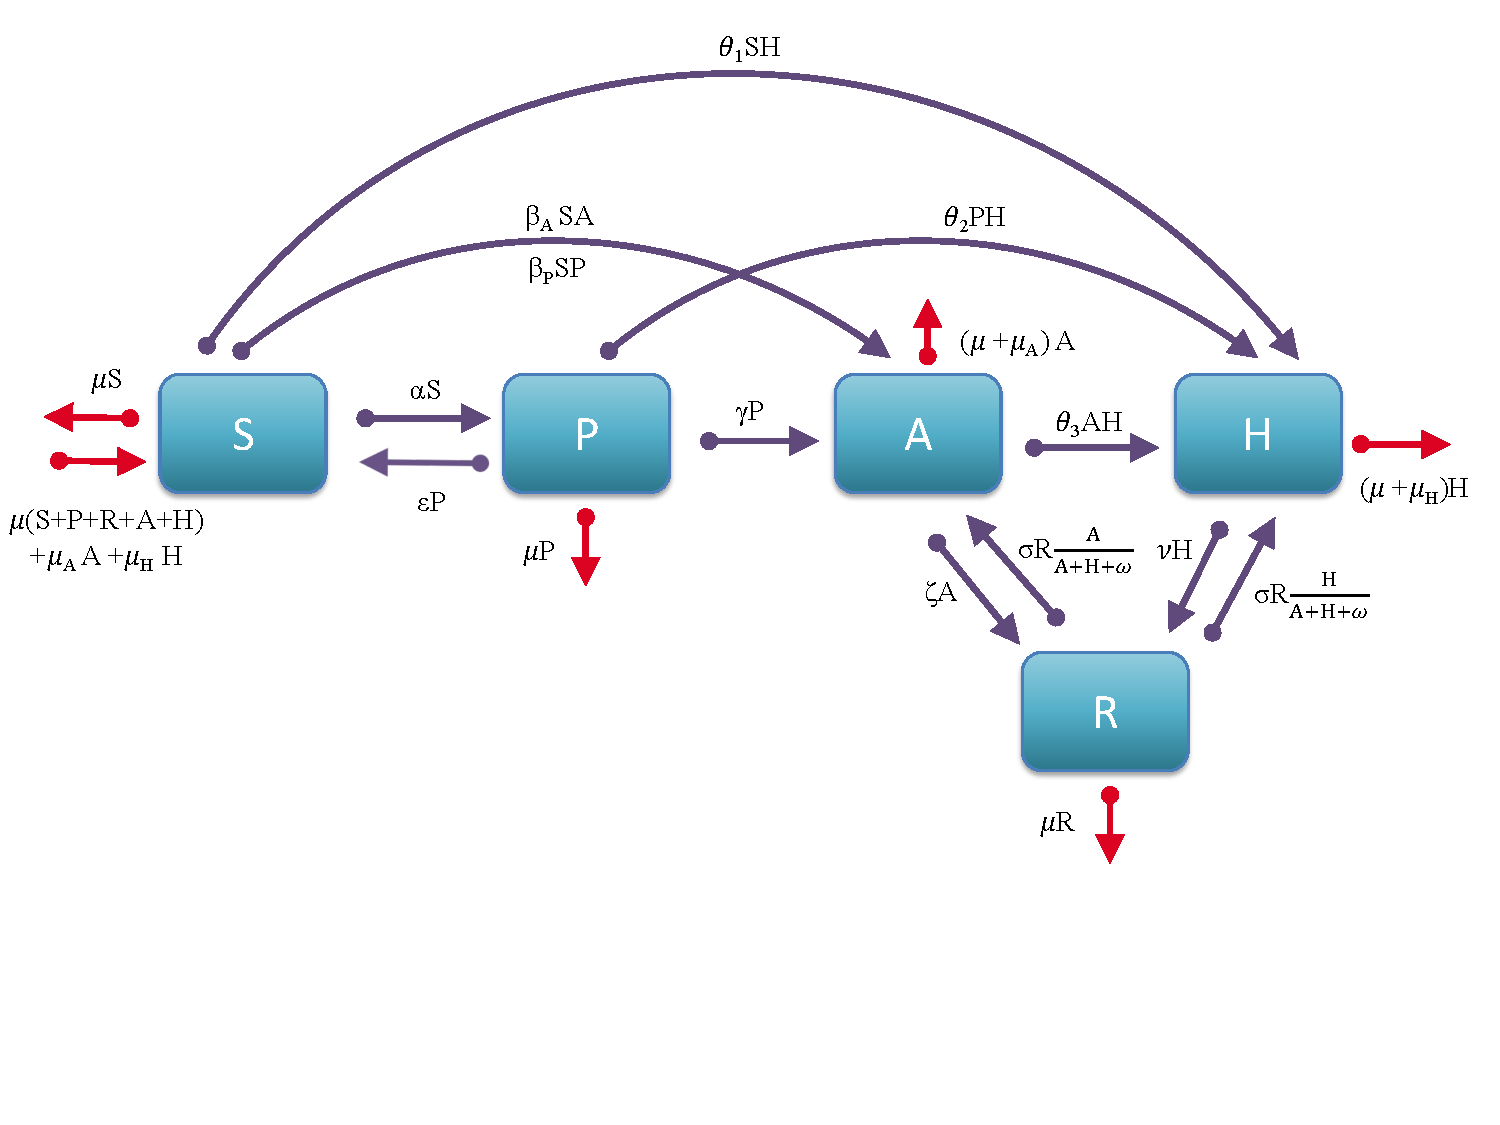
\includegraphics[scale=0.6]{heroin_schematic.pdf}
\vspace{-3cm}
\begin{center}
Figure 1: Schematic diagram for heroin model
\end{center}

 \textbf{Parameter Values} \\

\textcolor{red}{EDIT for local data in Knox County/Tennessee: May use ordinary least squares or bayseian inference since we are hoping to have data from experts--think about after NC State Parameter Estimation workshop; write program for data fitting} \\ 
We recognize that these estimated parameter values vary based on time and different locations within Knox County or East Tennessee, but are sufficient for analyzing the model. 
%The parameters for our model were estimated from the literature on opioids and heroin. 
%In 2015, individuals were prescribed opioids at a rate of 20.7 people out of 100, causing $\alpha=0.207$ [20].
%Need to fix$--$$>$It is estimated that eighty percent of those who use heroin misused prescription opioids in the past; we will make the assumption that individuals were addicted to opioids previously in order to estimate some parameters [30]. In 2015, there were 828,000 heroin users, meaning that 662,400 of them were addicted to prescription opioids [14]. Making the assumption that the chance of becoming a heroin user is equal among susceptible individuals and prescription opioid users, we will split the remaining 165,600 individuals into these two groups. In that case, 82,800 susceptible individuals becoming a heroin user out of a total population of 321,000,000 results in $\theta_{1}=0.0003$, and similarly for prescription opioids users, leading $\theta_{2}$ to be the same value. \\ 
%In 2011, a study was performed that resulted in a 90\% relapse rate to opioid use within one year after treatment ending, so that $\sigma_{A}=0.9$ [19]. \\
%We assume that individuals who go to treatment to deal with their addiction to opioids can only fall back into the opioid addiction class, and those who enter for heroin use only fall back into the heroin class. \\
%Based on $\sigma_{A}=0.9$ and $\sigma_{H}=$, this implied  $\delta=0.1$ + success from heroin , those who successfully ended their addiction to opioids [28, other ]. \\
%The death rate $\mu$ for the total population in 2015 was 2,712,630 people, or 0.84\%, which we make note includes opioid and heroin related deaths, as well [24]. \\
%The opioid overdose rate in 2015 was 4 out of 100,000 individuals, resulting in $\mu_A=.00004$, and similarly for $\mu_H$ [25]. \\
%Prescription opioid users become dependent on opioids at a rate of 26\%, resulting in $\gamma=0.26$ and $\epsilon=0.74$ [28]. \\
%Four percent of prescription opioid users start using heroin, leading to $\theta_3=.04$ and heroin users enter treatment at a rate of 15\% so that $\nu=.15$ [14].}


 \textbf{Proof of existence of solution to ODE system} \\
Will show existence of solution to my ODE system. \textcolor{red}{Prove a priori solution is bounded in finite time?}


\textbf{Proof of non-negative initial conditions guaranteeing non-negative solutions} \\
We will now show that starting with non-negative initial conditions, solutions for the system (1)-(5) are guaranteed to be non-negative for all time, using the following theorem which is an adaptation of Theorem 2.1 in \cite{Smith}: 
 
 \textbf{Theorem 1} (\cite{Smith}: adapted version of Theorem 2.1, Chapter 5) 
\begin{comment} / Brittany Stephenson's dissertation 
\end{comment}
 \textit{Assume that when $\phi \in \mathbb{R}^n$ satisfies $\phi \geq 0$ with $\phi_{i}(0)=0$ for some $i$, then $f_i(\phi) \geq 0$. Then, if $\phi \in \mathbb{R}^n$ satisfies $\phi \geq 0$, the solution of $x'(t)=f(x(t)), x(t_{0})=\phi$ where $f: \mathbb{C}$ $\rightarrow$ $\mathbb{R}^n$ continuous, $\mathbb{C} \subset \mathbb{R}^n$ open and $\phi \in \mathbb{R}^n$, satisfies $x(t) \geq 0$ for all $t \geq t_{0}.$}
 
 \textbf{Proof} Consider the vector of initial conditions in $\mathbb{R}^5$, $\phi = (S_0, P_0, A_0, H_0, R_0).$ Since each vector component represents a proportion of a population, $\phi \geq 0.$ \\
 
1) Assume $\phi = (0, P_0, A_0, H_0, R_0) \geq 0.$ Then, 
\begin{center}
$f_1(\phi)=\epsilon P_0 +\delta R_0 + \mu (P_0+R_0)+(\mu + \mu_A) A_0 + (\mu+\mu_H) H_0 \geq 0,$
\end{center}
since all parameters and variables are non-negative. 
 
2) Assume $\phi = (S_0, 0, A_0, H_0, R_0) \geq 0.$ Then, 
\begin{center}
$f_2(\phi)=\alpha S_0 \geq 0,$
\end{center}
since $\alpha$ and $S_0$ are non-negative. 

3) Assume $\phi = (S_0, P_0, 0, H_0, R_0) \geq 0.$ Then,
\begin{center}
$f_3(\phi)=\gamma P_0 +\sigma_A R_0 + \beta \xi S_0 P_0 \geq 0,$
\end{center}
since all parameters and variables are non-negative. 
 
4) Assume $\phi = (S_0, P_0, A_0, 0, R_0) \geq 0.$ Then,
\begin{center}
$f_4(\phi)=\sigma_H R_0 \geq 0,$
\end{center}
since $\sigma_H$ and $R_0$ are non-negative. 
 
5)  Assume $\phi = (S_0, P_0, A_0, H_0, 0) \geq 0.$ Finally,
\begin{center}
$f_5(\phi)=\zeta A_0 +\nu H_0 \geq 0,$
\end{center}
since all parameters and variables are non-negative. 

%Thus, whenever $\phi \geq 0$ and $\phi_i(0)=0$ for some $i$ $\implies$ $f_i(\phi) \geq 0$. Therefore, since $\phi \geq 0$,  then by Theorem 1, the solution $X(t)=(S(t), P(t), A(t), H(t), R(t)) \geq 0$ for all $t \geq 0$, as desired. \square
 
\textbf{Addiction-Free Equilibrium} 
\textcolor{red}{Was unable to solve for endemic equilibrium...need to eventually?}

To find the addiction-free equilibrium, we set equations (1)-(5) equal to zero and require that $A=H=R=0$ since these three compartments consist of individuals who are addiction to opioids or heroin. We are left with the system: \\
\[0=-\alpha S^* -\beta \xi S^* P^* + \epsilon P^* +\mu P^* \quad\]
\[0=\alpha S^* - \epsilon P^* -\gamma P^* - \mu P^* \quad\]
\[0=\gamma P^* + \beta \xi S^* P^*.   \quad\]



If $P^*=0$, then the only solution is $S^*=P^*=H^*=R^*=0$, but $S^*=P^*=H^*=R^*=1$ by assumption, so this is not possible. Thus, we will assume $P^* \neq 0. $ This forces $\gamma + \beta \xi S^* =0$ and since all of our parameters and variables are non-negative, then it must be $\gamma=0$ and either $\beta=0$ or $\xi=0$. We have that $\gamma=0$ means that individuals who are prescribed opioids cannot become addicted to opioids. In addition, $\xi=0$ means that only black market opioids are available and there are no excess prescription drugs available and  $\beta=0$ means that susceptibles are unable to become addicted to opioids at all. We claim that $\beta=0$ is less realistic than the former since eliminating two paths to addiction from the susceptible class is less realistic than just eliminating one path. Under the assumption that $\gamma=0=\xi$ to ensure the existence of our addiction-free equilibrium and that $1=S+P+A+H+R$, we calculate the addiction-free equilibrium to be: \\

\[S^*=\frac{\epsilon + \mu}{\alpha + \epsilon +\mu}\quad\]
\[P^*=\frac{\alpha}{\alpha + \epsilon +\mu}\quad\]
\[A^*=0\quad\]
\[H^*=0\quad\]
\[R^*=0\quad\] 

Note that enforcing $P^* \neq 0$ implies that $\alpha \neq 0$, as well, which means that individuals are still able to be prescribed opioids. 

\textbf{Basic Reproduction Number, \textbf{$\mathscr{R}_0$}}

The basic reproduction number, denoted $\mathscr{R}_0$, is a term used in epidemiological models that gives the expected number of secondary disease cases that result from the introduction of a disease to a susceptible population. The value of $\mathscr{R}_0$ represents how successful the spread of the disease is expected to be; if $\mathscr{R}_0 < 1$, then the disease is expected to die out and the disease-free equilibrium will be locally stable; conversely, if $\mathscr{R}_0 >1$, then the disease is expected to spread and the disease-free equilibrium will be unstable \cite{Driessche}. \\ \\
 This idea may be applied to the context of our model since for the addiction-free equilibrium to occur, $\gamma=0$ and $\xi=0$, so that individuals can become addicted only with interactions with opioid addicted individuals or heroin users so takes the form of an infectious disease. Thus, in this case in which the prescription part is essentially taken out of the model so that it is a black-market-only driven model, $\mathscr{R}_0$ can be calculated. This value will be the ratio of the number of new addictions in the next year compared to the current year. At the addiction-free equilibrium, the population is completely susceptible, as needed for $\mathscr{R}_0$ to be an accurate measurement of addiction potential. 
We note that our goal in this section is to explore the structure of the model and not obtain a result for the full model. The disease compartments are those that contain infected individuals, or in our case, addicts \cite{Driessche}. Our model incorporates three addiction compartments, A, H, and R, since these all consist of opioid and/or heroin addicted individuals. We will utilize the Next Generation Matrix Method in order to calculate $\mathscr{R}_0$.


For the purposes of calculating $\mathscr{R}_0$, we will assume $\gamma =0$ and $\xi =0$ (thus, $\beta \neq 0$) in order to ensure the existence of the addiction-free equilibrium. This results in the following system:
\[\dv{S}{t} = -\alpha S - \beta SA  - \theta_{1} SH +\epsilon P +\delta R +\mu (P+R) + (\mu+\mu_{A})A + (\mu+\mu_{H}) H \quad \] 
\[\dv{P}{t} = \alpha S - \epsilon P  - \theta_{2}PH- \mu P    \quad\]
\[\dv{A}{t} = \sigma_{A} R +\beta SA  -\zeta A - \theta_{3}AH-(\mu + \mu_{A})A   \quad\]
\[\dv{H}{t} = \theta_{1}SH+\theta_{2}PH+\theta_{3}AH + \sigma_{H}R-\nu H-(\mu+\mu_{H})H  \quad\]
\[\dv{R}{t} = \zeta A +\nu H -\delta R -\sigma_{A}R-\sigma_{H}R -\mu R.\quad\]


In general, the differential equations of the $n$ disease compartments, $x_i'$, may be written as: 

\[{x_i'} = \mathscr{F}_{i} (x,y)-\mathscr{V}_i (x,y),\quad i=1,...,n\] 

where $x$ is a vector with the disease compartments as components, $y$ a vector with the non-disease compartments as components, $\mathscr{F}_{i}$ represents the rate that secondary infections contribute to disease compartment $i$ and $\mathscr{V}_{i}$ represents the rate of transitions, i.e. rate at which the disease compartment $i$ is decreased by means of death, recovery and progression of the disease for $i=1,2,3$ \cite{Driessche}. 

Thus, for our three addicted compartments, we may write: 

$$\dfrac{dA}{dt} = \mathscr{F}_{1} (x,y)-\mathscr{V}_{1}(x,y)$$
$$\dfrac{dH}{dt} = \mathscr{F}_{2} (x,y)-\mathscr{V}_{2}(x,y)$$
$$\dfrac{dR}{dt} = \mathscr{F}_{3} (x,y)-\mathscr{V}_{3}(x,y),$$

where $x= {[A\quad H\quad R]}^{T}$ and $y= {[S\quad P]}^{T}$.



Thus, under the assumption that A, H and R are the addicted compartments and abiding by the parameter restrictions stated above, the assumptions of the Next Generation Method are satisfied for matrices $\mathscr{F}$ and $\mathscr{V}$ formulated here:

\begin{center}
$\mathscr{F}=$
$ \begin{pmatrix}

\beta SA \\
\theta_{1}SH+\theta_{2}PH \\
0
\end{pmatrix}$



$\mathscr{V}=$
$ \begin{pmatrix}

-\sigma_{A}R+\zeta A+\theta_{3} AH + (\mu +\mu_{A})A \\
-\theta_{3}AH-\sigma_{H}R+\nu H +(\mu +\mu_{H}) H \\
-\zeta A -\nu H +\delta R +\sigma_{A}R +\sigma_{H}R +\mu R\\
\end{pmatrix}$.
\end{center}

These assumptions include the following: 
\begin{itemize}
\item $\mathscr{F}_{i} (0,y)=0$ and $\mathscr{V}_{1}(0,y)=0$,  $\forall$$y \geq 0$, $i=1,2,3$, which ensures that new addictions arise only from interacting with those currently addicted, and there is no immigration into the addicted compartments; these guarantee that the population free of addiction remains that way. 
\item $\mathscr{F}_{i} (x,y) \geq 0$, $\forall$$x,y \geq 0$, $i=1,2,3$ since these represent new addictions. 
\item $\mathscr{V}_{i}(x,y) \leq 0$ whenever $x_i=0, i=1,2,3$ since there must be inflow only when the respective compartment is empty. 
\item $\sum_{n=1}^{3} \mathscr{V}_{i}(x,y) \geq 0$, $\forall x,y \geq 0$ since this represents the total outflow from all addicted compartments. 
\item The addiction-free system, $\dv{S}{t}\bigg|_{A,H,R=0}$ and $\dv{P}{t}\bigg|_{A,H,R=0}$ has a unique equilibrium, ($\frac{\epsilon+\mu}{\alpha+\epsilon+\mu}$,$\frac{\alpha}{\alpha+\epsilon+\mu}$) that is asymptotically stable. 
\end{itemize}

Taking $F=\frac{\partial \mathscr{F}_i}{\partial x_j} (0, y_0)$ and $V=\frac{\partial \mathscr{V}_i}{\partial x_j} (0, y_0)$, $i, j =1, 2, 3$, where (0, $y_{0}$) $=(\frac{\epsilon + \mu}{\alpha + \epsilon +\mu},\frac{\alpha}{\alpha + \epsilon +\mu},0,0,0)$ is the addiction-free equilibrium, we calculated the following \cite{Driessche}: 



\begin{center}
$F=$
$ \begin{pmatrix}

\beta S^* &  0  & 0 \\
0 & \theta_1 S^* +\theta_2 P^* & 0\\
0  &   0 & 0\\
\end{pmatrix}$



$V=$
$ \begin{pmatrix}

\zeta +\mu +\mu_A &  0  & -\sigma_A \\
0 &  \nu+\mu+\mu_H & -\sigma_H\\
-\zeta& -\nu  & \delta + \sigma_A + \sigma_H + \mu\\

\end{pmatrix}$.
\end{center}

The eigenvalues of $FV^{-1}$ are calculated to be: 
\begin{center}
$\sigma (FV^{-1}) = \{0, \frac{(r+s)-\sqrt{(r-s)^2+4\beta S^* z  \sigma_A \zeta \sigma_H \nu}}{2det(V)} 
, \frac{(r+s)+\sqrt{(r-s)^2+4\beta S^* z  \sigma_A \zeta \sigma_H \nu}}{2det(V)} 
\}$
\end{center}

where $a=\zeta +\mu + \mu_A$, $b=\nu + \mu + \mu_H$, $c=\delta + \sigma_A + \sigma_H +\mu$, $z=\theta_1 S^* + \theta_2 P^*$, $ r=\beta S^* (bc-\sigma_H \nu), s=z(ac-\sigma_{A} \zeta)$, and $det(V)=a(bc-\sigma_H\nu)-\sigma_A\zeta b$.

$\mathscr{R}_0$ may then be determined as the spectral radius of $FV^{-1}$, in which the $(i,j)$ entry is the expected number of secondary addictions in compartment $i$ produced by individuals initially in compartment $j$ :
\begin{center}
$\mathscr{R}_0=$ $\frac{(r+s)+\sqrt{(r-s)^2+4\beta S^* z  \sigma_A \zeta \sigma_H \nu}}{2det(V)}. $
\end{center}

This value is the spectral radius since it is the largest eigenvalue greater than 0. We can see this by first noting that the radicand $(r-s)^2+4\beta S^* z  \sigma_{A} \zeta \sigma_{H} \nu$ is positive, since all parameters are positive. In addition, $r$ is positive because in the multiplication of $bc=\delta \mu + \delta \nu+ \delta \mu_{H}+ \mu^{2} + \mu \nu+ \mu \mu_{H} + \mu \sigma_{A} + \mu \sigma_{H}+ \nu \sigma_{A}+$ \hl{$ \sigma_{H} \nu $} $+ \mu_{H}\sigma_{A}+\mu_{H}\sigma_{H}$, all terms are positive and the highlighted term cancels with $-\sigma_{H} \nu$, leaving only a positive sum. Multiplying by $\beta S^*$, the resulting value $r$ is positive. Similarly, $s$ is positive because in the multiplication of $ac=\delta \mu_{A} + \delta \mu + \delta \zeta + \mu_{A} \mu+ \mu_{A} \sigma_{A}+\mu_{A} \sigma_{H} +\mu^{2} +\mu \zeta+ \mu \sigma_{A}+\mu \sigma_{H}+$ \hl{$\sigma_{A} \zeta$} $+ \zeta \sigma_{H}$, all terms are positive and the highlighted term cancels with $-\sigma_{A} \zeta$, again resulting in a sum of only positive terms. Multiplied against positive value $z$, this results in $s$ being positive. Finally, the expansion of $det(V)$ is positive. This is because $bc$ is a positive sum containing a term that cancels with $-\sigma_{H} \nu$ as described above and $ac$ shown above contains the term $\sigma_{A} \zeta$ which multiplied with b cancels with $-\sigma_A\zeta b,$ thus resulting in a positive determinant. \textcolor{red}{Need to prove AFE is stable if $\mathscr{R}_0$ $<$ 1 and unstable if $>$ 1?}

%Don't include, most likely: Increasing $\beta$ (the rate of addiction via non-prescription means), $\theta_1$ (the rate of heroin addiction of the susceptible population), and $\theta_2$ (the rate of heroin addiction of the prescribed population), all increase $\mathscr{R}_0$ since these parameters only appear in the numerator of $\mathscr{R}_0$, specifically within the $r$, $z$, and $s$ terms. \\ 

\textbf{Sensitivity Analysis} \\
\textcolor{red}{Planning to use Sobol, read more about, and maybe think about others, such as Latin Hypercube/ PRCC? Do we need local sensitivity analysis at all? Info: https://www.mathworks.com/help/sldo/ug/what-is-sensitivity-analysis.html , https://www.mathworks.com/help/sldo/ug/sampling-parameters-and-states.html  } 

In order to explore the sensitivity of each of the population classes to each of the parameters, we implemented Sobol sensitivity analysis in which the Saltelli sampler is utilized to generate N(2D+2) parameter samples where N$=$FILL IN is the number of sample points and D=16, the number of parameters in the model for a total of FILL IN samples \cite{Herman}. 
Saltelli are the statistically good points chosen in the parameter space to test and records S, P, A, H and R at the final time (t=10 years) for the parameter choices. Samples N points from the problem and returns a matrix of parameter values. 
%Think about why N(2D+2) and why N(D+2) for taking out second order interactions. 
\textcolor{red}{Look into total order indices: total variance (sum?), expectation (variance), normalized sum. Look at Saltelli reference, equation 44: term+complement+interaction terms} \\
\textcolor{red}{Once have baseline parameters, do +/- 50\% for each parameter and cut off $\mu$ so does not go all the way to 0?}
Both $\mu_{A}$ and $\mu_{H}$ were restricted to the domain $[0,0.1]$ with the remaining parameters ranging on the entire domain $[0,1]$. For first-order indices, only one parameter is varied and the rest are held constant; for second-order indices, two parameters are varied and the rest are held constant; and for total-order indices, every combination of parameters is varied, from a single parameter varying alone to all higher-order interactions between parameters. The length of the colored bars, with each color representing a specific class, measures the contribution of a certain parameter to the variance of each of the classes in the model. The longer the colored bar, the higher the effect the parameter has on that class of individuals. We are able to retrieve the confidence intervals on the sensitivity of each of the populations to a respective change in the parameter(s) for first order changes, second order changes and total order changes. \\
\textcolor{red}{Change time step to -1: result[0][-1] I believe, because want to see how outputs (S,P,A,H,R) are affected at the FINAL time}

%Add in sensitivity analysis results and confidence interval information once converges 
%Takes the mean from the last 100 (or 10 for the case of t=10) time steps. (I thought final time??) \\
%Total --take average of all interactions for plots?? \\
%Need to scale sensitivities of muA and muH based on their domain $[0,0.1]$??

%Per Lenhart--use sensitivity analysis results to parse out different pieces of information; such as integrate \alphaP to get all new addiction individuals??
\textbf{Future Work/Ideas} 


-Obtain local data from Knox County/East Tennessee, can calculate $\mathscr{R}_0$ from there (would expect $<$ 1 b/c prescriptions seem to be a huge driving force behind addiction to opioids and individuals switching to heroin use. Contact with Davide Stern (UT hospital), Paul Erwin, Agricola Odoi, Kelly Cooper\\
-Perform sensitivity analysis to determine the sensitivity of each of the classes to the parameters (i.e. the contribution of each of the parameters to the sizes of the classes). Plan to use Sobol sensitivity analysis in which the saltelli sampler is utilized to generate (statistically good) parameter samples. Will only perform on the full  odel, not the AFE b/c that would require $t$ very large and we want to look at shorter term, such as $t=10$ years. Will perform first, second and total indices. \\
-Fit parameters to data that are difficult to find in literature. \\
-Explore management strategies for how to best treat pain with prescriptions while reducing opioid addiction and heroin use (optimal control or scenario analysis).  \\
Possible extentions: \\
-Break recovery class into two different classes for opioid addicts and heroin users (look at pain management and why people relapse: START paper and Addiction Treatment Study). \\
-Look into gender, race, socioeconomic class, incarceration or rural versus urban location to investigate differences; treatment programs/types of treatment/success rates (see Modeling Gender Differences in Drug Abuse Epidemics paper, paper copy in desk and Length of Stay in Different Drug Using States: Lifestyles of Problem and Recreational Drug Consumers for location, also see "future papers to read" in heroin folder)% (examples in Christopher's work for gender: women more likely to have chronic pain, be prescribed opioids, be given higher doses an use them for longer than men CDC 2013, but men are twice as likely to overdose on opioids 2016...and race: white/non-hispanic significantly more likely to overdose on opioids than black/non-hispanic or hispanic) 
-Significance of naloxone for reversing effects of overdose 
-Consider Markov Chain model (Lou from oral exam) 
-Linda Allen slides from Stochastic Modeling of Biological and Ecological Systems 2018 MN workshop 
\\ \\
For a paper: \textit{Acknowledgements: The authors would like to thank Dr. Nicholas Battista and Leigh Pearcy for their contributions.}

\pagebreak

\textcolor{red}{Currently working on cleaning up citations} 
\bibliography{HeroinModel}

%\printbibliography


 \end{document}
